\begin{figure}[h] 
\centering 
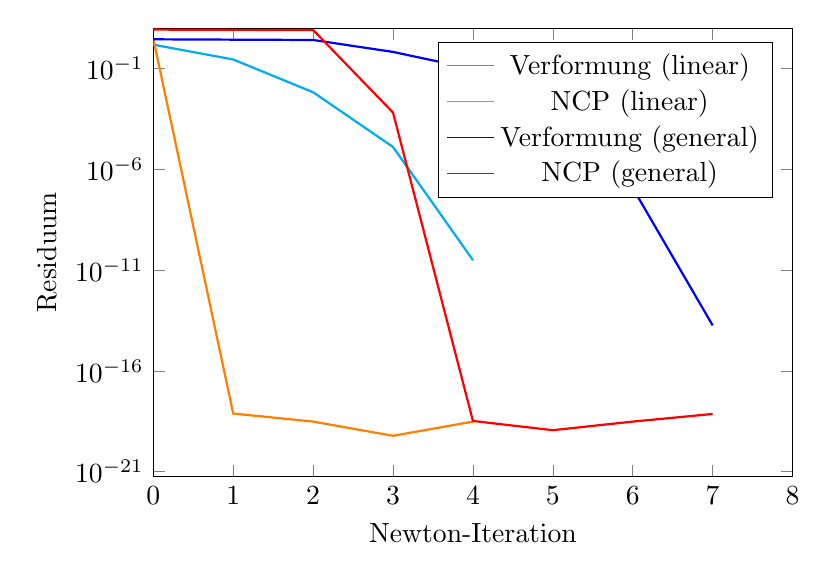
\begin{tikzpicture}[every plot/.append style={thick}] 
\begin{axis}[ 
label style={font=\normalsize}, 
xlabel={Newton-Iteration}, 
ylabel={Residuum}, 
xmin=0, xmax=8, 
ymode=log, 
ymin=0, ymax=10, 
width=0.8\textwidth, 
height=0.6\textwidth, 
legend pos=north east, 
legend style={cells={align=left}}, 
grid style=dashed, 
] 
\addplot[ 
color=cyan, 
] 
coordinates { 
(0, 1.53e+00)(1, 2.82e-01)(2, 6.69e-03)(3, 1.29e-05)(4, 3.14e-11)}; 
\addlegendentry{Verformung (linear)} 
\addplot[ 
color=orange, 
] 
coordinates { 
(0, 3.02e+00)(1, 7.72e-19)(2, 3.07e-19)(3, 6.06e-20)(4, 3.07e-19)}; 
\addlegendentry{NCP (linear)} 
\addplot[ 
color=blue, 
] 
coordinates { 
(0, 2.82e+00)(1, 2.71e+00)(2, 2.61e+00)(3, 6.67e-01)(4, 9.52e-02)(5, 9.55e-04)(6, 1.19e-07)(7, 1.81e-14)}; 
\addlegendentry{Verformung (general)} 
\addplot[ 
color=red, 
] 
coordinates { 
(0, 8.56e+00)(1, 8.29e+00)(2, 8.21e+00)(3, 6.56e-04)(4, 3.30e-19)(5, 1.15e-19)(6, 3.07e-19)(7, 7.34e-19)}; 
\addlegendentry{NCP (general)} 
\end{axis} 
\end{tikzpicture} 
\caption{Residuen des Stoffgesetzes 'Neo Hooke' mit Hinderniss 'Hut' und 2178 Freiheitsgraden für die Verschiebung.} 
\label{fiq:NeoHooke_Hut_level4} 
\end{figure} 
